\documentclass[handout]{beamer} % Use the beamer class for presentations, 'handout' option to suppress \pause

\input{Lecture-Slides/preamble.txt}

% Define the transition slide command
\newcommand{\transitionslide}[1]{
    \begin{frame}[plain]
        \centering
        \vspace{1cm}
        \Huge
        \textcolor{moonstoneblue!150}{\textbf{#1}}
    \end{frame}
}

% Title and Author Info
\title{Introduction to Statistical Methods in Political Science}
\subtitle{Lecture 5: Random Variables, PMF, PDF, and CDF}
\author{Ignacio Urbina \texorpdfstring{\\ \vspace{0.3em}}{ } \scriptsize \textcolor{gray}{Ph.D. Candidate in Political Science}}
\date{}

%%%%%%%%%%%%%%%%%%%%%%%%%%%%%%%%%%%%%%%%%%%%%%%%%%%%%%%%%%%%%%%%%%%%%%%%%%%%%%
%%% DATA


%%%%%%%%%%%%%%%%%%%%%%%%%%%%%%%%%%%%%%%%%%%%%%%%%%%%%%%%%%%%%%%%%%%%%%%%%%
%%% BEGIN DOC
%%%%%%%%%%%%%%%%%%%%%%%%%%%%%%%%%%%%%%%%%%%%%%%%%%%%%%%%%%%%%%%%%%%%%%%%%%

\begin{document}
\frame{\titlepage}

%%%%%%%%%%%%%%%%%%%%%%%%%%%%%%%%%%%%%%%%%%%%%%%%%%%%%%%%%%%%%%%%%%%%%%%%%%
\section{Random Variables and their Probability Distributions}
\transitionslide{Random Variables and their Probability Distributions}

% Slide 2: From Events to Numbers
\begin{frame}
    \frametitle{From Events to Numbers}
    \begin{itemize}
        \item Previously, we studied the probability of discrete events, such as: \pause
        \begin{itemize}
            \item Probability of two countries going to war. \pause
            \item Probability that a Senator is a woman. \pause
            \item Probability that a randomly sampled person a bachelor's degree. \pause
            \item Probability of getting an even number when throwing a die.  \pause
        \end{itemize}
        \item These probabilities help us understand the likelihood of events. \pause
        \item To perform deeper statistical analysis, we need to quantify these events numerically. 
    \end{itemize}
\end{frame}

% Slide 3: Transforming Educational Attainment into Numbers
\begin{frame}
    \frametitle{Transforming Educational Attainment into Numbers}
    \begin{itemize}
        \item For example, consider educational attainment levels: \pause
        \begin{itemize}
            \item No education \pause
            \item Incomplete high school \pause
            \item Complete high school \pause
            \item Some college \pause
            \item Bachelor's degree \pause
            \item Graduate degree \pause
        \end{itemize}
        \item Instead of discrete categories, we can measure the number of years of schooling. \pause
        \item This allows us to calculate statistics like the mean number of years of education. 
    \end{itemize}
\end{frame}

% Slide 4: The Need for Quantification
\begin{frame}
    \frametitle{Continuous Numerical Variables: Feeling Thermometers}
    \begin{itemize}
        \item Consider the feeling thermometer used in surveys like the American National Elections Study (\href{https://electionstudies.org/}{ANES}): \pause
        \begin{itemize}
            \item Rate feelings toward political figures on a scale from 0 to 100. \pause
            \item 0 = Very cold or unfavorable \pause
            \item 50 = Neutral \pause
            \item 100 = Very warm or favorable \pause
        \end{itemize}
        \item This allows us to calculate statistics like mean favorability. 
    \end{itemize}
\end{frame}

% Slide 5: Introduction to Random Variables
\begin{frame}
    \frametitle{Introduction to Random Variables}
    \begin{itemize}
        \item We use \textbf{random variables} to numerically quantify events. \pause
        \item A random variable assigns a numerical value to each outcome in a sample space. \pause
        
    \definitionbox{Random Variable $(Def.)$}{A random variable is a function that maps each outcome in the sample space $S$ to a specific numeric value.} \pause
    
        \item Allows us to quantify events and analyze them numerically. \pause
        \item \textbf{In practice, we treat Random Variables as numeric variables} and manipulate them using specific algebra rules.
        \item Example: Tossing a coin, where heads are assigned a 1, and tails a 0. \pause
    \end{itemize}


    
\end{frame}

% Slide 6: Types of Random Variables
\begin{frame}
    \frametitle{Types of Random Variables}
    \begin{itemize}
        \item \textbf{Discrete Random Variables} \pause
        \begin{itemize}
            \item Take on a finite or countable number of values. \pause
            \item Example: Number of children in a family, number of votes received by a candidate. \pause
        \end{itemize}
        \item \textbf{Continuous Random Variables} \pause
        \begin{itemize}
            \item Take on an infinite number of values within a given range. \pause
            \item Example: Income level, time spent on social media. \pause
        \end{itemize}
    \end{itemize}
\end{frame}

% Slide 7: Random Variables for One Die
\begin{frame}
    \frametitle{Random Variables for One Die}
    \begin{itemize}
        \item Define the sample space \( S \) for throwing one die as: \pause
        \[
        S = \{1, 2, 3, 4, 5, 6\}
        \]  \pause \vspace{-1.5em}
        \item Define a random variable \( X \) as a function 
            \[ X: S \rightarrow \{1, 2, 3, 4, 5, 6\} \]. \pause \vspace{-1.5em}
        \item \( X \) maps each outcome in the sample space to a numerical value. \pause
        \item Let $X=x$ be a specific value of $X$. Examples: \pause
        \begin{itemize}
            \item If the die shows 2, then \( x = 2 \). \pause
            \item If the die shows 5, then \( x = 5 \). \pause
            \item If the die shows 1, then \( x = 1 \). \pause
        \end{itemize}
    \end{itemize}
\end{frame}

% Slide 8: Random Variables for Two Dice
\begin{frame}
    \frametitle{Random Variables for Two Dice}
    \begin{itemize}
        \item Define the sample space \( S \) for two dice as: \pause
        \begin{align*}
        S &= \big\{(i, j) \mid i, j \in \big\{1, 2, 3, 4, 5, 6\big\}\big\} \\
          &= \big\{(1,1), (1,2), (1,2), \cdots, (2,1), (2,2), \cdots, (6,5), (6,6)\big\}    
        \end{align*}
        \pause \vspace{-1.5em}
        \item The sum of the two dice numbers can be represented by a random variable \( Z \). \pause
        \item Let $Z=z$ be a specific value of $Z$. Examples: \pause
        \begin{itemize}
            \item If the dice show (2, 3), then \( z = 2 + 3 = 5 \). \pause
            \item If the dice show (6, 1), then \( z = 6 + 1 = 7 \). \pause
            \item If the dice show (4, 4), then \( z = 4 + 4 = 8 \). \pause
            \item If the dice show (3, 5), then \( z = 3 + 5 = 8 \). \pause
        \end{itemize}
    \end{itemize}
\end{frame}

% Slide 8: Random Variables for Two Dice
\begin{frame}
    \frametitle{Random Variables for Two Dice}
    \begin{itemize}
        \item Depending on \textbf{how we define an event, the function used as a random variable will change}.
        \item Define the sample space \( S \) for two dice as: \pause
        \begin{align*}
        S &= \big\{(i, j) \mid i, j \in \big\{1, 2, 3, 4, 5, 6\big\}\big\} \\
          &= \big\{(1,1), (1,2), (1,3), \cdots, (2,1), (2,2), \cdots, (6,5), (6,6)\big\}    
        \end{align*} \pause \vspace{-1.5em}
        \item The \myemph{total number of even dice obtained from throwing two dice} can be represented by a random variable \( V \). \pause
        \item Let $V=v$ be a specific value of $V$. Examples: \pause
        \begin{itemize}
            \item If the dice show (2, 3), then \( v = 1 + 0 = 1 \). \pause
            \item If the dice show (1, 6), then \( v = 0 + 1 = 1 \). \pause
            \item If the dice show (4, 4), then \( v = 1 + 1 = 2 \). \pause 
            \item If the dice show (3, 5), then \( v = 0 + 0 = 0 \). \pause
        \end{itemize}
    \end{itemize}
\end{frame}


% Slide 9: Random Variables for One Coin
\begin{frame}
    \frametitle{Random Variables for One Coin}
    \begin{itemize}
        \item Define the sample space \( S \) for throwing a coin as: \pause
        \begin{align*}
        S = \big\{H, T\big\}    
        \end{align*} \pause \vspace{-1.5em}
        \item Define a random variable \( W \) as a function \( W: S \rightarrow \{0, 1\} \), where \( W \) represents the number of heads. \pause
        \item \( W \) maps each outcome in the sample space to the number of heads. \pause
        \item Examples: \pause
        \begin{itemize}
            \item If the coin shows H, then \( w = 1 \). \pause
            \item If the coin shows T, then \( w = 0 \). \pause
        \end{itemize}
    \end{itemize}
\end{frame}

% Slide 10: Random Variables for Three Coins
\begin{frame}
    \frametitle{Random Variables for Three Coins}
    \begin{itemize}
        \item Define the sample space \( S \) for three coins as: \pause
        \begin{align*}
        S =& \big\{ (H, H, H), (H, H, T), (H, T, H), (H, T, T), (T, H, H),  \\
        & (T, H, T), (T, T, H), (T, T, T) \big\}
        \end{align*}  
        \vspace{-1.7em}
        \pause
        \item Define a random variable \( Y \) as a function \( Y: S \rightarrow \{0, 1, 2, 3\} \), where \( Y=y \) represents the number of heads. \pause
        \item \( Y \) maps each outcome in the sample space to the number of heads. \pause
        \item Examples: \pause
        \begin{itemize}
            \item If the coins show (H, H, T), then \( y = 2 \). \pause
            \item If the coins show (T, T, T), then \( y = 0 \). \pause
            \item If the coins show (H, H, H), then \( y = 3 \). \pause
            \item If the coins show (T, H, T), then \( y = 1 \). 
        \end{itemize}
    \end{itemize}
\end{frame}

% Slide 11: Random Variables for Election Results
\begin{frame}
    \frametitle{Random Variables for Election Results}
    \begin{itemize}
        \item Consider the results of the last Senatorial election in three battleground states. Define the sample space \( S \) for these results as: \pause \vspace{-1em}
        \begin{align*}
        S =& \big\{ (R, R, R), (R, R, D), (R, D, R), (R, D, D), (D, R, R),\\
        & (D, R, D), (D, D, R), (D, D, D) \big\}
        \end{align*} \pause \vspace{-2.5em}
        \item Define a random variable \( Z \) as a function \( Z: S \rightarrow \{0, 1, 2, 3\} \), where \( Z=z \) represents the number of battleground states won by the Republican Party. \pause
        \item \( Z \) maps each outcome in the sample space to the number of states won by the Republican Party. \pause
        \item Examples: \pause
        \begin{itemize}
            \item If the results are (R, R, D), then \( z = 2 \). \pause
            \item If the results are (D, D, D), then \( z = 0 \). \pause
            \item If the results are (R, R, R), then \( z = 3 \). \pause
            \item If the results are (D, R, D), then \( z = 1 \). \pause
        \end{itemize}
    \end{itemize}
\end{frame}


% Slide 12: Definition of Probability for Discrete Random Variables
\begin{frame}
    \frametitle{Definition of Probability for Discrete Random Variables}

    
    \definitionbox{Probability for Discrete Random Variables $(Def.)$}{
    When each outcome in the sample space \( S \) is equally likely, the probability that a discrete random variable \( X \) takes the value \( x \) is given by the ratio of the number of outcomes in \( S \) where \( X = x \) to the total number of outcomes in \( S \).
    } \pause 

    \begin{itemize}
        \item For a discrete random variable \( X \) and a specific value \( x \): \pause
        \[
        P(X = x) = \frac{\text{Number of favorable outcomes in which } X = x}{\text{Total number of possible outcomes}} 
        \] \pause \vspace{-1.0em}
        \item This is based on the classical definition of probability \pause
    \end{itemize}
\end{frame}

%* THE FOLLOWING IS WRONG mist be P(X)

% Slide 11: Axioms of Probability for Random Variables
\begin{frame}
\frametitle{Properties of the Probability Distribution for a Discrete Random Variable}

A function can serve as the probability distribution for a discrete random variable \( X \) if and only if its values, \( P(X=x) \), satisfy the conditions:
\pause  \vspace{1.0em}
    \begin{itemize}
        \item \( P(X=x) \geq 0 \) for each value within its domain \pause \vspace{1.0em}
        \item \( \sum_{i =1}^{k} P(X=x_i) = 1 \), where the summation extends over all the values within its domain ($\mathcal{D}_X = \{x_1, x_2, \cdots, x_k\}$) \pause \vspace{1.0em}
    \end{itemize}

Note that a \emph{discrete} random variable's probability distribution is often referred to as its \textbf{Probability Mass Function (PMF)}.

\end{frame}


% Slide 13: Probability Distribution for Number of Heads in Three Coin Tosses
\begin{frame}
    \frametitle{Probability Distribution for Number of Heads in Three Coin Tosses}
    \begin{itemize}
        \item Sample space \( S \) for three coin tosses: \pause
        \begin{align*}
        S =& \big\{ (H, H, H), (H, H, T), (H, T, H), (H, T, T), (T, H, H), \\\
        & (T, H, T), (T, T, H), (T, T, T) \big\}
        \end{align*} 
        \vspace{-1.7em}
        \pause
        \item Define random variable \( X \) as the number of heads. \pause
        \item Probability Distribution (PMF): 
        \begin{table}
            \centering
            \begin{tabular}{|c|c|}
                \hline
                \textbf{Number of Heads: $x$} & \textbf{Probability: $P(X=x)$} \\
                \hline
                0 & \( 1/8 \) \pause \\
                1 & \( 3/8 \) \pause \\
                2 & \( 3/8 \) \pause \\
                3 & \( 1/8 \) \pause \\
                \hline
            \end{tabular}
        \end{table}
    \end{itemize}
\end{frame}


% Slide 2: Introduction to 10-Point Feeling Thermometer
\begin{frame}
\frametitle{Example: Simplified Feeling Thermometer}
    \begin{itemize}
        \item Suppose a survey firm implemented a 10-point feeling thermometer to measure people's feelings towards political leaders or public figures.
        \pause
        \item Ratings range from 0 (very unfavorable) to 10 (very favorable).
        \pause
        \item Let's say this pollster was interested in the feelings towards the current President among the public.
        \pause
        \item Define the random variable \( X \) as the response of one subject on this thermometer.
    \end{itemize}
\end{frame}


% Slide 3: PMF and Probability Questions
\begin{frame}
\frametitle{PMF for the 10-Point Feeling Thermometer Towards the Current President ($x$)}
    \begin{minipage}[t]{0.3\linewidth}
        \textbf{PMF for \( X \)} \\
        \begin{tabular}{c|c}
            \toprule
            \( x \) & \( P(X=x) \) \\
            \midrule \pause 
            0 & 0.05 \\
            1 & 0.10 \\
            2 & 0.10 \\
            3 & 0.15 \\
            4 & 0.10 \\
            5 & 0.15 \\
            6 & 0.10 \\
            7 & 0.10 \\
            8 & 0.05 \\
            9 & 0.05 \\
            10 & 0.05 \\
            \bottomrule 
        \end{tabular} \pause 
    \end{minipage}%
    \begin{minipage}[t]{0.55\linewidth}

        \textbf{Probability Questions}

\small
What is the probability that  $X$ is... \newline 
1. Greater than or equal to 8? \newline \vspace{-1.5em} \pause 
\begin{align*}
   & P(X \geq 8) = P(X=8) + P(X=9) + P(X=10) \\[0.1em]  
   & = 0.05 + 0.05 + 0.05 = 0.15. \\[-2em] 
\end{align*} \pause 
2. Less than 5?  \newline \vspace{-1.5em} \pause 
\begin{align*}  
   & P(X < 5) = \\[0.1em]
   & = p_X(0) + p_X(1) + p_X(2) + p_X(3) + p_X(4) \\[0.1em]
   & = 0.05 + 0.10 + 0.10 + 0.15 + 0.10 = 0.50. \\[-2em]  
\end{align*} \pause 
3. Between 3 and 7 inclusive?  \newline \vspace{-1.5em} \pause 
\begin{align*}  
   & P(3 \leq X \leq 7) = P(X=3) + P(4) + \cdots + P(7) \\
   & = 0.15 + 0.10 + 0.15 + 0.10 + 0.10 = 0.60.
\end{align*}

\end{minipage}
\end{frame}

{\setbeamertemplate{footline}{}
\begin{frame}[noframenumbering]
\frametitle{}
\centering
\vspace*{\fill}
{\color{moonstoneblue!170}\usebeamerfont{title}\textbf{\Large Common PMF For Discrete Random Variables}}
\vspace*{\fill}
\end{frame}
}


% Slide 4: Common PMFs for Discrete Random Variables
\begin{frame}
\frametitle{Common PMFs for Discrete Random Variables}
    \begin{itemize}
        \item There are several common probability mass functions (PMFs) used to model discrete random variables. \pause
        \item We will discuss three of them: \pause
        \begin{itemize}
            \item Uniform Distribution \pause
            \item Bernoulli Distribution \pause
            \item Binomial Distribution
        \end{itemize}
        \item But note that there are several more: Negative Binomial, Geometric, Poisson, Multinomial, etc (see: \href{https://online.stat.psu.edu/stat504/lesson/1/1.3}{Link}).
        \item The following is a strongly recommended reference: \url{https://uw-statistics.github.io/Stat311Tutorial/discrete-distributions.html}.
    \end{itemize}
\end{frame}

% Slide 5: Uniform Distribution
\begin{frame}
\frametitle{Uniform Distribution}
    \begin{itemize}
        \item In a uniform distribution, each outcome is equally likely. \pause
        \item For a discrete random variable \( X \) with \( n \) possible outcomes: \pause
        \[
        p_X(x) = \frac{1}{n} \quad \text{for all } x
        \] \pause
        \item Note that: $p_X(x)\geq0$ and $\sum_x p_X(x) = \frac{1}{n} + \frac{1}{n} + \cdots + \frac{1}{n} = n \times \frac{1}{n} = 1 $
        \item This means that $p_X(x)$ is a well-defined PMF.
    \end{itemize}
\end{frame}

% Slide 6: Example: Uniform Distribution
\begin{frame}
\frametitle{Example: Uniform Distribution}
    \begin{itemize}
        \item Consider rolling a fair six-sided die: \pause
        \[
        S = \{1, 2, 3, 4, 5, 6\}
        \] \pause
        \item The PMF for each outcome is: \pause
        \[
        p_X(x) = \frac{1}{6} \quad \text{for } x = 1, 2, 3, 4, 5, 6
        \] \pause
        \item This means each number has an equal probability of \( \frac{1}{6} \).
    \end{itemize}
\end{frame}

% Slide 7: More examples.
\begin{frame}
\frametitle{Calculating Probabilities for Events Involving a Fair Six-Sided Die}
    \begin{itemize}
        \item \textbf{Single Value Event:} \pause
        \begin{itemize}
            \item Probability of rolling a 4: \pause
            \[
            P(X = 4) = \frac{1}{6}
            \]
        \end{itemize}
        
        \item \textbf{Composite Event:} \pause
        \begin{itemize}
            \item Probability of rolling an even number (2, 4, or 6): \pause
            \[
            P(x \text{ is even}) = P(X = 2) + P(X = 4) + P(X = 6) = \frac{1}{6} + \frac{1}{6} + \frac{1}{6} = \frac{3}{6}
            \]
        \end{itemize}
        
        \item \textbf{Multiple Disjoint Events:} \pause
        \begin{itemize}
            \item Probability of rolling a number less than 4 (1, 2, or 3): \pause
            \[
            P(x < 4) = P(X = 1) + P(X = 2) + P(X = 3) = \frac{1}{6} + \frac{1}{6} + \frac{1}{6} = \frac{3}{6} = \frac{1}{2}
            \]
        \end{itemize}

        \item \textbf{Non-occurring Event:} \pause
        \begin{itemize}
            \item Probability of rolling a 7: \pause
            \[
            P(x = 7) = 0
            \]
        \end{itemize}
    \end{itemize}
\end{frame}

% Slide 8: Bernoulli Distribution
\begin{frame}
\frametitle{Bernoulli Distribution}
    \begin{itemize}
        \item The Bernoulli distribution models a single trial with two outcomes: success (1) and failure (0). \pause
        \item For a random variable \( X \) with success probability \( p \): \pause
        \[
        p_X(x) = \begin{cases} 
        p & \text{if } x = 1 \\
        1 - p & \text{if } x = 0
        \end{cases}
        \] \pause
        \item Which of the two outcomes is labeled as a success or failure is generally arbitrarily defined.
    \end{itemize}
\end{frame}

% Slide 9: Example: Bernoulli Distribution
\begin{frame}
\frametitle{Example: Bernoulli Distribution}
    \begin{itemize}
        \item Consider flipping a fair coin: \pause
        \[
        S = \{H, T\}
        \] \pause
        \item Let \( X \) be 1 if heads (H) and 0 if tails (T). If the coin is fair, the PMF is: \pause
        \[
        p_X(x) = \begin{cases} 
        0.5 & \text{if } x = 1 \\
        0.5 & \text{if } x = 0
        \end{cases}
        \]
    \end{itemize}
\end{frame}


% Slide 10: Example: Bernoulli Distribution for Sociodemographic Variable
\begin{frame}
\frametitle{Example: Bernoulli Distribution for Sociodemographic Variable}
    \begin{itemize}
        \item \textbf{Example}: If we randomly select one person among the American public, what is the probability they identify as Latino/a/x? \pause
        \item Let \( X \) be a random variable where \( X = 1 \) if the person identifies as Latino/a/x and \( X = 0 \) otherwise. \pause
        \item According to 2020 US Census data, the probability \( p \) that a randomly selected person identifies as Latino/a/x is 0.189. \pause
        \item We can represent $X$ as a Bernoulli random variable : \pause
        \[
        p_X(x) = \begin{cases} 
        0.189 & \text{if } x = 1 \\
        0.811 & \text{if } x = 0
        \end{cases}
        \] \pause
    \end{itemize}
\end{frame}

% Slide 7: Binomial Distribution
\begin{frame}
\frametitle{Binomial Distribution}
    \begin{itemize}
        \item The binomial distribution models the number of successes in a fixed number of independent Bernoulli trials. \pause
        \item For a random variable \( X \) representing the number of successes in \( n \) trials with success probability \( p \): \pause
        \[
        p_X(x) = \binom{n}{x} p^x (1-p)^{n-x}
        \] \pause
        \item Example: Number of heads in 10 flips of a fair coin.
    \end{itemize}
\end{frame}

% Slide 8: Example: Binomial Distribution
\begin{frame}
\frametitle{Example: Binomial Distribution}
    \begin{itemize}
        \item Consider flipping a fair coin 10 times: \pause
        \[
        n = 10, \quad p = 0.5
        \] \pause
        \item The PMF for the number of heads \( X \) is: \pause
        \[
        p_X(x) = \binom{10}{x} (0.5)^x (0.5)^{10-x}
        \] \pause
        \item This gives the probability of getting exactly \( x \) heads in 10 flips.
    \end{itemize}
\end{frame}

% Slide : Example
\begin{frame}
\footnotesize
\frametitle{Example: Given a random sample of 10 people, what is the probability that two or fewer identify as Latino/a/x?}
    \begin{itemize}
        \setlength{\itemsep}{0pt} % Adjusts vertical spacing between items
        \item Define \( X \) as the number of Latinos in a sample of 10. This follows a binomial distribution: \( X \sim \text{Binomial}(N=10, p=0.189) \). \pause
        \[
        P(X = 0) = \binom{10}{0} \times 0.189^0 \times 0.811^{10} \approx 0.1231
        \] \pause
        \[
        P(X = 1) = \binom{10}{1} \times 0.189^1 \times 0.811^{9} \approx 0.2868
        \] \pause
        \[
        P(X = 2) = \binom{10}{2} \times 0.189^2 \times 0.811^{8} \approx 0.3008
        \] \pause
        \item Adding these probabilities:
        \[
        P(X \leq 2) = P(X = 0) + P(X = 1) + P(X = 2) \approx 0.7107
        \]
        \item This formula calculates the total probability of getting 0, 1, or 2 Latinos in the sample, which is approximately 71.07\%.
    \end{itemize}
\end{frame}

% Slide: Follow-up Probability Calculation
\begin{frame}
\footnotesize
\frametitle{Example: Probability of at least 1 or at least 3 Latinos in a sample of 10}
    \begin{itemize}
        \setlength{\itemsep}{0pt} % Adjusts vertical spacing between items
        \item Define \( X \) as the number of Latinos in a sample of 10. This follows a binomial distribution: \( X \sim \text{Binomial}(N=10, p=0.189) \). \pause
        
        \item \textbf{Probability of at least 1 Latino:} \pause
        \[
        P(X \geq 1) = 1 - P(X = 0)
        \]
        \[
        P(X \geq 1) = 1 - 0.1231 \approx 0.8769
        \]
        
        \item \textbf{Probability of at least 3 Latinos:} \pause
        \[
        P(X \geq 3) = 1 - P(X \leq 2)
        \]
        \[
        P(X \geq 3) = 1 - 0.7107 \approx 0.2893
        \]
        
        \item These probabilities show that there is an 87.69\% chance of having at least one Latino in the sample and a 28.93\% chance of having at least three.
    \end{itemize}
\end{frame}


\begin{frame}
\frametitle{Galton Board and the Binomial Distribution}
\begin{itemize}
    \item Binomial PMF graph: \url{https://shiny.rit.albany.edu/stat/binomial/}
    \item Galton Board: \url{https://www.mathsisfun.com/data/quincunx.html}
\end{itemize}
\end{frame}

{\setbeamertemplate{footline}{}
\begin{frame}[noframenumbering]
\frametitle{}
\centering
\vspace*{\fill}
{\color{moonstoneblue!170}\usebeamerfont{title}\textbf{\Large Probability for Continuous Random Variables}}
\vspace*{\fill}
\end{frame}
}




% Slide: Concept of Probability for Continuous Random Variables
\begin{frame}
\frametitle{Concept of Probability for Continuous Random Variables}
    \begin{itemize}
        \item Continuous random variables take on infinite possible values within a given range. \pause
        \item Therefore, the probability of \emph{exactly} obtaining a specific value $X=x$ after a random trial is $0$ due to this definition. \pause
        \item Hence, when dealing with \textbf{continuous random variables}, we need to work with \textbf{probabilities of intervals}, i.e., $\Pr(X \in [a,b])$. \pause
        \item So, instead of asking what's the probability that someone's height is precisely 5 feet 7.16 inches, we can ask what is the probability that someone's height is between 5 feet 5 inches and 5 feet 10 inches.
    \end{itemize}
\end{frame}

% Slide: Introduction to Probability Density Function (PDF)
\begin{frame}
\frametitle{Introduction to Probability Density Function (PDF)}
    \begin{itemize}
        \item The \textbf{Probability Density Function (PDF)}, denoted as $f_X(x)$, describes the likelihood of a continuous random variable $X$ taking on a particular value. \pause
        \item Note: the PDF represents the \emph{relative likelihood} of $X$ being near $x$. $f_X(x)$ \textbf{IS NOT} the probability of $x$.  \pause
        \item To find the probability that $X$ lies within an interval $[a, b]$, we calculate the area under the PDF curve between $a$ and $b$. \pause
        \item Mathematically, this is formally expressed using definite integrals:
        \[
        P(X\in [a,b]) = P(a \leq X \leq b) = \int_{a}^{b} f_X(x) \, \cdot dx
        \] 
    \end{itemize}
\end{frame}


% Slide: Intuition of Definite Integrals
\begin{frame}
\frametitle{Notation: Definite Integrals (\emph{optional slide})}
    \begin{itemize}
        \item A definite integral represents the area under the graph of a function and the x-axis. \pause
        \item The notation for a definite integral is:
        \[
        \int_{a}^{b} f(x) \, \cdot dx
        \] \pause \vspace{-1.5em}
        \item Here:
        \begin{itemize}
            \item \(a\) is the lower limit of integration.
            \item \(b\) is the upper limit of integration.
            \item \(f(x)\) is the function being integrated.
            \item \(dx\) indicates that the integration is with respect to \(x\).
        \end{itemize} \pause
        \item The definite integral calculates the net area between the function \(f(x)\) and the x-axis from \(x = a\) to \(x = b\).
    \end{itemize}
\end{frame}

% Slide: Definition of a Well-Defined PDF
\begin{frame}
\frametitle{Definition of a Well-Defined Probability Density Function (PDF)}
\vspace{0.5em}

\definitionbox{Probability Density Function (PDF)}{
A function $f_X(x)$ is a valid probability density function (PDF) of a continuous random variable $X$ if and only if it satisfies the non-negativity and normalization conditions.
}

\begin{enumerate}
    \item \textbf{Non-Negativity:} For all possible values of $x$,
    \[
    f_X(x) \geq 0, \quad \text{for all } x.
    \]
    \pause
    \item \textbf{Normalization:} The total probability over all possible values of $X$ must sum to 1, meaning:
    \[
    \int_{-\infty}^{\infty} f_X(x) \,dx = 1.
    \]
\end{enumerate}


\end{frame}



% Slide: Connecting the Dots with a Random Variable (Two-Column Layout)
\begin{frame}
\frametitle{Connecting the Dots: Example}

\begin{columns}
    % First Column: Description (1/3 of the slide width)
    \column{0.33\textwidth}
    \begin{itemize}
        \item Define a random variable $X$ that takes values from 0 to 2. \pause
        \item The PDF of $X$ follows a \emph{triangular distribution} with mode at $c=1$: \pause
        \[
        f_X(x) =
        \begin{cases}
        x, & 0 \leq x \leq 1 \\
        (2-x), & 1 \leq x \leq 2
        \end{cases}
        \] \pause
    \end{itemize}

    % Second Column: Graph (2/3 of the slide width)
    \column{0.67\textwidth}
    \begin{center}
    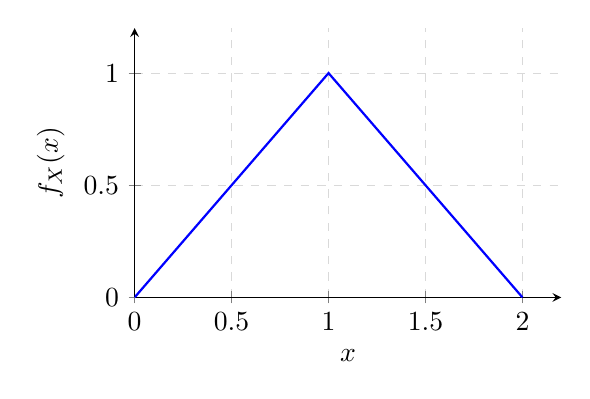
\begin{tikzpicture}
        \begin{axis}[
            axis lines = left,
            xlabel = {$x$},
            ylabel = {$f_X(x)$},
            domain=0:2,
            samples=100,
            xmin=0, xmax=2.2,
            ymin=0, ymax=1.2,
            grid = major,
            width=7cm,  % Adjusted width
            height=5cm, % Adjusted height
            grid style={dashed, gray!30}
        ]
        % Plot the triangular distribution
        \addplot[blue, thick] coordinates {(0,0) (1,1) (2,0)};
        % Labels
        \node at (axis cs:1,-0.2) [anchor=north] {$1$};
        \node at (axis cs:2,-0.2) [anchor=north] {$2$};
        \node at (axis cs:-0.1,2) [anchor=east] {$2$};
        \end{axis}
    \end{tikzpicture}
    \vspace{4.5em}
    \end{center}
\end{columns}

\end{frame}


% Slide: Area Under the Curve of the PDF
\begin{frame}
\frametitle{Area Under the Curve of the PDF}
    \begin{itemize}
        \item The area under the PDF consists of two right triangles. \pause
        \item The left triangle (from $0$ to $1$) has:
        \begin{itemize}
            \item Base = $1-0=1$
            \item Height = $1$
        \end{itemize} \pause
        \item The right triangle (from $1$ to $2$) has:
        \begin{itemize}
            \item Base = $2-1=1$
            \item Height = $1$
        \end{itemize} \pause
        \item Using the formula for the area of a triangle:
        \[
        \left(\frac{1}{2} \times 1 \times 1\right) + \left(\frac{1}{2} \times 1 \times 1\right) = 0.5+0.5= 1
        \] \pause
        \item This confirms the total area under the curve is 1, making it a valid PDF.
    \end{itemize}
\end{frame}

% Slide: Calculating Probability for an Interval
\begin{frame}
\frametitle{Calculating Probability for an Interval}
\textbf{Problem:} Calculate the probability that $X$ lies between $0.5$ and $1$.  \pause
    \begin{itemize}
        \item The probability is the area under the PDF between $0.5$ and $1$, which can be broken down as the area of a small triangle and a rectangle under $f_X(x)$ from $0.5$ to $1.0$. \pause
        \item Rectangle area:
        \begin{itemize}
            \item Base = $1 - 0.5 = 0.5$ \pause
            \item Height = $0.5 - 0 = 0.5$ \pause
            \item Area = $Base \times Height  = 0.5\times 0.5 = 0.25$
        \end{itemize}
        \item Small triangle area: 
        \begin{itemize}
            \item Base = $1 - 0.5 = 0.5$ \pause
            \item Height = $1 - 0.5 = 0.5$ \pause
            \item Area = $\dfrac{1}{2}\times Base \times Height  = \dfrac{1}{2}\times 0.5 \times 0.5= 0.125$
        \end{itemize}
        
        \item Thus,
        \[
        P(0.5 \leq X \leq 1) = 0.25 + 0.125 = 0.375
        \]
    \end{itemize}
\end{frame}


\begin{comment}
% Slide: Graph of 3x using TikZ
\begin{frame}
\frametitle{Graph of $f(x)=3x$}
    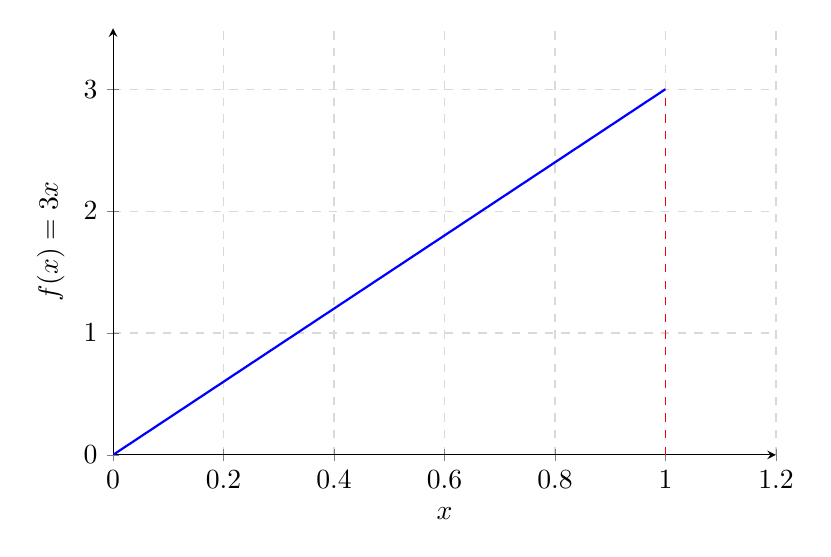
\begin{tikzpicture}
        \begin{axis}[
            axis lines = left,
            xlabel = {$x$},
            ylabel = {$f(x) = 3x$},
            domain=0:1,
            samples=100,
            xmin=0, xmax=1.2,
            ymin=0, ymax=3.5,
            grid = major,
            width=10cm,
            height=7cm,
            grid style={dashed, gray!30}
        ]
        % Plot the function
        \addplot[blue, thick] {3*x};
        % Add vertical line at x=1
        \addplot[dashed, red] coordinates {(1,0) (1,3)};
        % Label the points
        \node at (axis cs:1,-0.2) [anchor=north] {$1$};
        \node at (axis cs:-0.1,3) [anchor=east] {$3$};
        \end{axis}
    \end{tikzpicture}
\end{frame}

% Slide: Area Calculation of Triangle and Remarks

 

\begin{frame}
\frametitle{Area Under $f(x)=3x$}
    \begin{itemize}
        \item The area under the line \(3x\) between \(x=0\) and \(x=1\) forms a triangle. 
        \item The base of the triangle is \(1-0 = 1\). 
        \item The height of the triangle is \(3 \times 1 = 3\). 
        \item Using the formula for the area of a triangle:  \pause
        \[
        \text{Area} = \frac{1}{2} \times \text{base} \times \text{height} = \frac{1}{2} \times 1 \times 3 = \frac{3}{2}
        \] \pause
        \item This means:
        \[
        \int_{0}^{1} 3x \, \cdot dx = \frac{3}{2}
        \] 
    \end{itemize}
\end{frame}

% Slide: Area Calculation of Triangle and Remarks
\begin{frame}
\frametitle{Definite Integrals and Area Under the Curve}
    \begin{itemize}
        \item For the function $f(x)=3x$ the area under the curve (graph) between $0$ and $1$ is given by:
        \[
        \int_{0}^{1} 3x \, dx = \frac{3}{2}
        \] \pause
        \item \textbf{Remark 1:} This definite integral represents the area under the function \(3x\) from \(x=0\) to \(x=1\). \pause
        \item \textbf{Remark 2:} In this course, we will not manually solve integrals, as this requires calculus. When dealing with continuous random variables, we will use tables in which a computer has computed the area within important predefined intervals (more on this in the following weeks).
    \end{itemize}
\end{frame}
\end{comment}


% Slide: Connecting the Dots with a Random Variable
\begin{frame}
\frametitle{Example 2}
    \begin{itemize}
        \item Define a random variable \(X\) that takes on values from 0 to 2. \pause 
        \item Suppose the PDF of \(X\) is \(f_X(x) = \frac{1}{2}x\) for \(0 \leq x \leq 2\). \pause
        \item Graph of \(f_X(x) = \frac{1}{2}x\) from 0 to 2: \pause 
    \end{itemize}

    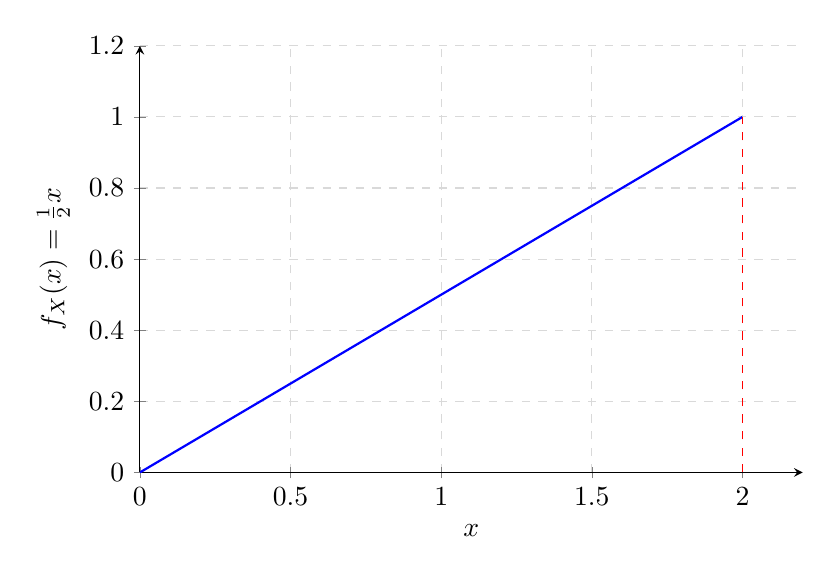
\begin{tikzpicture}
        \begin{axis}[
            axis lines = left,
            xlabel = {$x$},
            ylabel = {$f_X(x) = \frac{1}{2}x$},
            domain=0:2,
            samples=100,
            xmin=0, xmax=2.2,
            ymin=0, ymax=1.2,
            grid = major,
            width=10cm,
            height=7cm,
            grid style={dashed, gray!30}
        ]
        % Plot the function
        \addplot[blue, thick] {0.5*x};
        % Add vertical line at x=2
        \addplot[dashed, red] coordinates {(2,0) (2,1)};
        % Label the points
        \node at (axis cs:2,-0.2) [anchor=north] {$2$};
        \node at (axis cs:-0.1,1) [anchor=east] {$1$};
        \end{axis}
    \end{tikzpicture}
\end{frame}

% Slide: Showing the Area Under the Curve
\begin{frame}
\frametitle{Area Under the Curve of the PDF}
    \begin{itemize}
        \item The area under the curve \(f_X(x) = \frac{1}{2}x\) from \(x=0\) to \(x=2\) forms a right triangle.
        \item The base of the triangle is \(2-0 = 2\).
        \item The height of the triangle is \(\frac{1}{2} \times 2 = 1\). \pause 
        \item Using the formula for the area of a triangle: \pause 
        \[
        \text{Area} = \frac{1}{2} \times \text{base} \times \text{height} = \frac{1}{2} \times 2 \times 1 = 1
        \] \pause
        \item This means the total area under the PDF is 1, making it a well-defined PDF.
    \end{itemize}
\end{frame}

% Slide: Calculating the Probability for an Interval
\begin{frame}
\frametitle{Calculating Probability for an Interval}
    \begin{itemize}
        \item To calculate the probability that \(X\) lies between 0.5 and 1.5: \pause 
        \item We use one rectangle and one triangle to represent the area. \pause
    \end{itemize}

    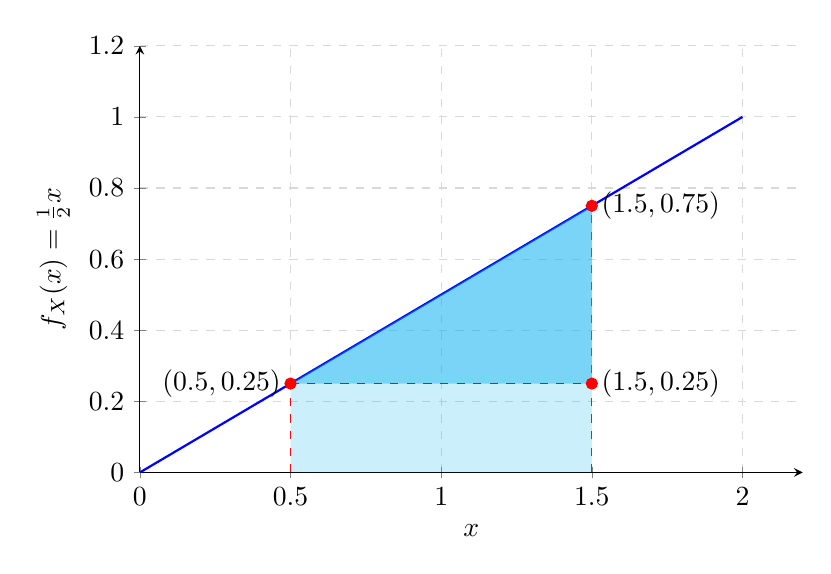
\begin{tikzpicture}
        \begin{axis}[
            axis lines = left,
            xlabel = {$x$},
            ylabel = {$f_X(x) = \frac{1}{2}x$},
            domain=0:2,
            samples=100,
            xmin=0, xmax=2.2,
            ymin=0, ymax=1.2,
            grid = major,
            width=10cm,
            height=7cm,
            grid style={dashed, gray!30}
        ]
        % Plot the function
        \addplot[blue, thick] {0.5*x};
        % Add vertical lines at x=0.5 and x=1.5
        \addplot[dashed, red] coordinates {(0.5,0) (0.5,0.25)};
        \addplot[dashed, red] coordinates {(1.5,0) (1.5,0.75)};
        % Fill the area under the curve from 0.5 to 1.5
        \addplot[draw=none, fill=cyan, fill opacity=0.2] coordinates {(0.5,0) (0.5,0.25) (1.5,0.75) (1.5,0)};
        % Fill the triangle area
        \addplot[draw=none, fill=cyan, fill opacity=0.4] coordinates {(0.5,0.25) (1.5,0.75) (1.5,0.25)};
        % Add red dashed line between (0.5, 0.25) and (1.5, 0.25)
        \addplot[dashed, red] coordinates {(0.5,0.25) (1.5,0.25)};
        % Add points at (0.5, 0.25), (1.5, 0.25), and (1.5, 0.75)
        \addplot[only marks, mark=*, red] coordinates {(0.5,0.25) (1.5,0.25) (1.5,0.75)};
        % Label the points with coordinates
        \node at (axis cs:0.5,0.25) [anchor=east] {$(0.5, 0.25)$};
        \node at (axis cs:1.5,0.25) [anchor=west] {$(1.5, 0.25)$};
        \node at (axis cs:1.5,0.75) [anchor=west] {$(1.5, 0.75)$};
        % Label the points on the x and y axis
        \node at (axis cs:0.5,-0.1) [anchor=north] {$0.5$};
        \node at (axis cs:1.5,-0.1) [anchor=north] {$1.5$};
        \node at (axis cs:-0.1,0.25) [anchor=east] {$0.25$};
        \node at (axis cs:-0.1,0.75) [anchor=east] {$0.75$};
        \end{axis}
    \end{tikzpicture}
    
\end{frame}

% Slide: Calculating the Probability for an Interval
\begin{frame}
\frametitle{Calculating Probability for an Interval}
 
    \begin{itemize}
        \item The area of the rectangle (base = 1.5 - 0.5 = 1, height = 0.25):
        \[
        \text{Area} = \text{base} \times \text{height} = 1 \times 0.25 = 0.25
        \] \pause 
        \item The area of the triangle (base = 1.5 - 0.5 = 1, height = 0.75 - 0.25 = 0.5):
        \[
        \text{Area} = \frac{1}{2} \times \text{base} \times \text{height} = \frac{1}{2} \times 1 \times 0.5 = 0.25
        \] \pause 
        \item Total area from 0.5 to 1.5:
        \[
        0.25 + 0.25 = 0.5
        \] \pause 
        \item This means:
        \[
        P(0.5 \leq X \leq 1.5) = \int_{0.5}^{1.5} \frac{1}{2}x \, \cdot dx = 0.5
        \]
    \end{itemize}
\end{frame}

% Slide 10: Example: Probability for Continuous Random Variables
\begin{frame}
\frametitle{Uniform Distribution for Continuous Random Variables}
    \begin{itemize}
        \item Consider the uniform distribution on the interval [0, 1]. \pause
        \item The PDF is: \pause
        \[
        f_X(x) = \begin{cases} 
        1 & \text{if } 0 \leq x \leq 1 \\
        0 & \text{otherwise}
        \end{cases}
        \] \pause
        \item The total area under the PDF curve is 1.
    \end{itemize}
\end{frame}

% Slide: Graph of the Uniform Distribution PDF
\begin{frame}
\frametitle{Graph of the Uniform Distribution PDF}
    \begin{tikzpicture}
        \begin{axis}[
            axis lines = left,
            xlabel = {$x$},
            ylabel = {$f_X(x)$},
            domain=-0.2:1.2,
            samples=100,
            ymin=0, ymax=1.2,
            grid = major,
            width=10cm,
            height=7cm,
            grid style={dashed, gray!30}
        ]
        % Plot the function
        \addplot[blue, thick] coordinates {(0,1) (1,1)};
        % Add vertical line at x=1
        \addplot[dashed, red] coordinates {(1,0) (1,1)};
        % Label the points
        \node at (axis cs:0,-0.1) [anchor=north] {$0$};
        \node at (axis cs:1,-0.1) [anchor=north] {$1$};
        \node at (axis cs:-0.1,1) [anchor=east] {$1$};
        \end{axis}
    \end{tikzpicture}
\end{frame}

% Slide: Calculating the Probability and Shaded Area
\begin{frame}
\frametitle{Probability Calculation for Uniform Distribution}
    \begin{itemize}
        \item The probability that \(X\) is greater than 0.75 in a uniform distribution from 0 to 1 is calculated as follows:
        \[
        P(0.75 < X) = 1 \times (1 - 0.75) = 0.25
        \]
    \end{itemize}
    
    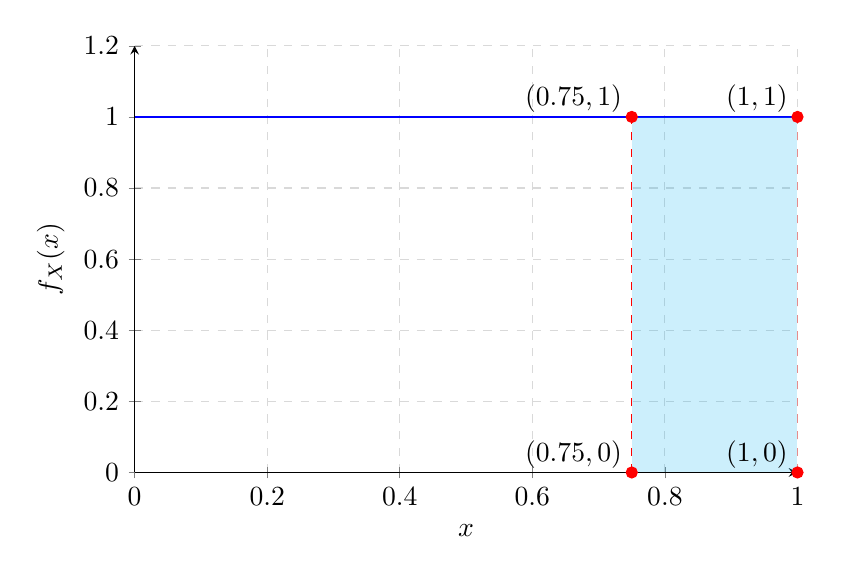
\begin{tikzpicture}
        \begin{axis}[
            axis lines = left,
            xlabel = {$x$},
            ylabel = {$f_X(x)$},
            domain=-0.2:1.2,
            samples=100,
            ymin=0, ymax=1.2,
            grid = major,
            width=10cm,
            height=7cm,
            grid style={dashed, gray!30}
        ]
        % Plot the function
        \addplot[blue, thick] coordinates {(0,1) (1,1)};
        % Add vertical line at x=1
        \addplot[dashed, red] coordinates {(1,0) (1,1)};
        % Add vertical line at x=0.75
        \addplot[dashed, red] coordinates {(0.75,0) (0.75,1)};
        % Fill the area under the curve from 0.75 to 1
        \addplot[draw=none, fill=cyan, fill opacity=0.2] coordinates {(0.75,0) (0.75,1) (1,1) (1,0)};
        % Add points at (0.75, 0), (0.75, 1), (1, 0), (1, 1)
        \addplot[only marks, mark=*, red] coordinates {(0.75,0) (0.75,1) (1,0) (1,1)};
        % Label the points with coordinates
        \node at (axis cs:0.75,0) [anchor=east, yshift=6.5pt] {$(0.75, 0)$};
        \node at (axis cs:0.75,1) [anchor=east, yshift=6.5pt] {$(0.75, 1)$};
        \node at (axis cs:1,0) [anchor=east, yshift=6.5pt] {$(1, 0)$};
        \node at (axis cs:1,1) [anchor=east, yshift=6.5pt] {$(1, 1)$};
        \end{axis}
    \end{tikzpicture}
\end{frame}

{\setbeamertemplate{footline}{}
\begin{frame}[noframenumbering]
\frametitle{}
\centering
\vspace*{\fill}
{\color{moonstoneblue!170}\usebeamerfont{title}\textbf{\Large Introduction to the Normal Distribution}}
\vspace*{\fill}
\end{frame}
}


% Slide 11: Normal Distribution
\begin{frame}
\frametitle{Normal Distribution}
    \begin{itemize}
        \item The normal distribution is a continuous probability distribution. \pause
        \item Defined by its mean \( \mu \) and standard deviation \( \sigma \). \pause
        \item The PDF of the normal distribution is: \pause
        \[
        f_X(x) = \frac{1}{\sqrt{2\pi\sigma^2}} e^{-\frac{(x-\mu)^2}{2\sigma^2}}
        \]
        \item Main features of the normal distribution: \pause
        \begin{itemize}
            \item It is a symmetrical distribution.
            \item Values close to the mean are more likely than values very far from it.
        \end{itemize}
    \end{itemize}
\end{frame}

% Slide 12: Example: Normal Distribution
\begin{frame}
\frametitle{Example: Standard Normal Distribution}
    \begin{itemize}
        \item Consider a normal distribution with \( \mu = 0 \) and \( \sigma = 1 \) (standard normal distribution). \pause
        \item The PDF is: \pause
        \[
        f_X(x) = \frac{1}{\sqrt{2\pi}} e^{-\frac{x^2}{2}}
        \] \pause
        \item The total area under the PDF curve is 1.
    \end{itemize}
\end{frame}

% Slide: Graph of the standard normal
\begin{frame}
\begin{figure}[ht]
\centering
\begin{tikzpicture}
    \begin{axis}[
        domain=-4:4, 
        samples=100, 
        axis lines=middle, 
        xlabel=$x$, 
        ylabel={$f_X(x)$},
        every axis y label/.style={at=(current axis.above origin),anchor=south},
        every axis x label/.style={at=(current axis.right of origin),anchor=west},
        height=7cm, 
        width=12cm,
        xtick={-4,-3,...,4},
        ytick=\empty,
        enlargelimits=false, 
        clip=false, 
        axis on top,
        grid = major,
        grid style={dashed, gray!30}
    ]
        \addplot [
            very thick,
            cyan!50!black,
        ] {1/sqrt(2*pi) * exp(-x^2 / 2)};
        \node[below] at (axis cs: 0,0) {$0$};
    \end{axis}
\end{tikzpicture}
\caption{Standard Normal Distribution}
\end{figure}
\end{frame}

% Slide: Graph of Multiple Normal Distributions
\begin{frame}
\begin{figure}[ht]
\centering
\begin{tikzpicture}
    \begin{axis}[
        domain=-7:7, % Expanded x-axis range
        samples=100, 
        axis lines=middle, 
        xlabel=$x$, 
        ylabel={$f_X(x)$},
        every axis y label/.style={at=(current axis.above origin),anchor=south},
        every axis x label/.style={at=(current axis.right of origin),anchor=west},
        height=0.8\textheight, % Adjust height based on text height
        width=\linewidth, % Fit the width of the slide
        xtick={-7,-6,...,7},
        ytick=\empty,
        enlargelimits=false, 
        clip=false, 
        axis on top,
        grid = major,
        grid style={dashed, gray!30},
        legend style={at={(0.8,0.97)},anchor=north west,font=\tiny,inner sep=1pt} % Moved legend box to the left inside the graph
    ]
        % Standard Normal Distribution (mu = 0, sigma = 1)
        \addplot [
            very thick,
            cyan!50!black,
        ] {1/sqrt(2*pi) * exp(-x^2 / 2)};
        \addlegendentry{$\mu=0$, $\sigma=1$}

        % Normal Distribution (mu = -3, sigma = 1)
        \addplot [
            very thick,
            red,
        ] {1/sqrt(2*pi) * exp(-(x+3)^2 / 2)};
        \addlegendentry{$\mu=-3$, $\sigma=1$}

        % Normal Distribution (mu = 2, sigma = 1)
        \addplot [
            very thick,
            green!50!black,
        ] {1/sqrt(2*pi) * exp(-(x-2)^2 / 2)};
        \addlegendentry{$\mu=2$, $\sigma=1$}

        \node[below] at (axis cs: 0,0) {$0$};
    \end{axis}
\end{tikzpicture}
\caption{Comparison of Normal Distributions with Different Means}
\end{figure}
\end{frame}

% Slide: Graph of Multiple Normal Distributions with Same Mean, Different SD
\begin{frame}
\begin{figure}[ht]
\centering
\begin{tikzpicture}
    \begin{axis}[
        domain=-7:7, % Suitable range to show all distributions
        samples=100, 
        axis lines=middle, 
        xlabel=$x$, 
        ylabel={$f_X(x)$},
        every axis y label/.style={at=(current axis.above origin),anchor=south},
        every axis x label/.style={at=(current axis.right of origin),anchor=west},
        height=0.8\textheight, % Adjust height based on text height
        width=\linewidth, % Fit the width of the slide
        xtick={-7,-6,...,7},
        ytick=\empty,
        enlargelimits=false, 
        clip=false, 
        axis on top,
        grid = major,
        grid style={dashed, gray!30},
        legend style={at={(0.03,0.97)},anchor=north west,font=\tiny,inner sep=1pt} % Legend in the upper left corner inside the graph
    ]
        % Standard Normal Distribution (mu = 0, sigma = 1)
        \addplot [
            very thick,
            cyan!50!black,
        ] {1/sqrt(2*pi*1) * exp(-x^2 / (2*1))};
        \addlegendentry{$\mu=0$, $\sigma=1$}

        % Normal Distribution (mu = 0, sigma = 0.25)
        \addplot [
            very thick,
            red,
        ] {1/sqrt(2*pi*0.25) * exp(-x^2 / (2*0.25))};
        \addlegendentry{$\mu=0$, $\sigma=0.25$}

        % Normal Distribution (mu = 0, sigma = 4)
        \addplot [
            very thick,
            green!50!black,
        ] {1/sqrt(2*pi*4) * exp(-x^2 / (2*4))};
        \addlegendentry{$\mu=0$, $\sigma=4$}

        \node[below] at (axis cs: 0,0) {$0$};
    \end{axis}
\end{tikzpicture}
\caption{Comparison of Normal Distributions with Same Mean and Different Standard Deviations}
\end{figure}
\end{frame}

{\setbeamertemplate{footline}{}
\begin{frame}[noframenumbering]
\frametitle{}
\centering
\vspace*{\fill}
{\color{moonstoneblue!170}\usebeamerfont{title}\textbf{\Large Cumulative Distribution Function}}
\vspace*{\fill}
\end{frame}
}


\begin{frame}
\frametitle{Cumulative Distribution Function (CDF): Concept}

\begin{itemize}
  \item The Cumulative Distribution Function (CDF) is a function that describes the probability that a random variable takes a value less than or equal to a specific value.
  \pause
  \item It provides a complete description of the probability distribution of a random variable.
  \pause
  \item The CDF is fundamental in probability theory and statistics as it gives an integral overview of the distribution and helps in understanding the likelihood of different outcomes.
\end{itemize}

\end{frame}

\begin{frame}
\frametitle{Cumulative Distribution Function (CDF): Formal Definition}

\begin{columns}

\column{0.5\textwidth}
\textbf{Discrete Random Variable (RV)}
\begin{itemize}
    \item Definition: \vspace{0.7em}
\end{itemize}
  \pause
\small{\[
    F_X(x) = P(X \leq x) = \sum_{k: k \leq x} p_X(k)
\]}
  \pause
\begin{itemize}
    \item Here, $p_X(k)$ represents the probability mass function (PMF) of $X$ at $k$.
    \item For here and after we will denote $F_X(x)$ by $CDF_X(x)$.
\end{itemize}
  \pause

\vspace{-3em}
\column{0.5\textwidth}
\textbf{Continuous Random Variable (RV)}
\begin{itemize}
    \item Definition: 
  \pause
\end{itemize}
\small{
\[
  F_X(x) = P(X \leq x) = \int_{-\infty}^x f_X(t) \, dt
\]}
  \pause
\begin{itemize}
    \item $f_X(t)$ is the probability density function (PDF) of $X$. 
    \item For here and after we will denote $F_X(x)$ by $CDF_X(x)$.
\end{itemize}

\end{columns}

\end{frame}

%%%%%%%%%%%%%%%
\begin{frame}{Example of CDF for a Discrete RV}

\begin{columns}

\column{0.3\textwidth} %%%%%%%%%%%%%% COL 1
\footnotesize
\begin{itemize}
  \item \(X\) =  consecutive elections won by current members of the House of Representatives, with values from 1 to 10.
  \pause
  \item We define a left-skewed PMF for \(X\) where each \(p_X(x)\) decreases as \(x\) increases, reflecting a higher probability for fewer election wins.
  \pause
\end{itemize}

\column{0.7\textwidth} %%%%%%%%%%% COL 2
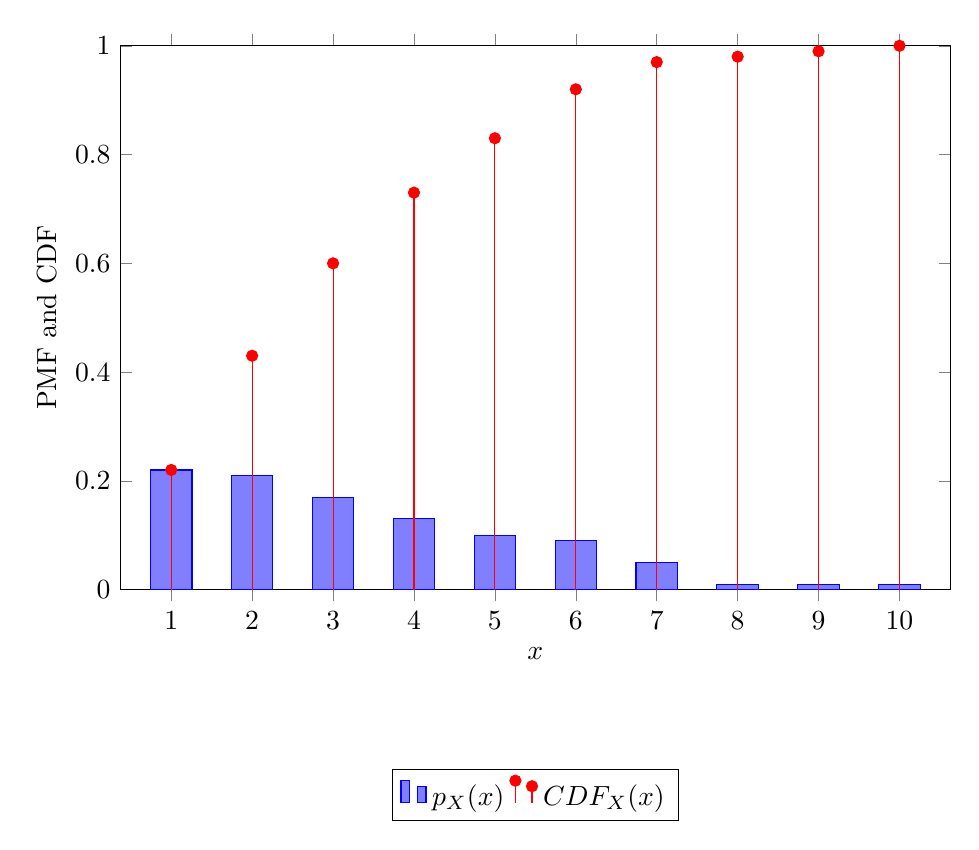
\begin{tikzpicture}[scale=1] % Adjust scale if needed
  % Draw PMF and CDF
  \begin{axis}[
    ybar, 
    bar width=15pt,
    xlabel={$x$},
    ylabel={PMF and CDF},
    symbolic x coords={1,2,3,4,5,6,7,8,9,10},
    xtick=data,
    ymin=0, ymax=1, % Adjust y-axis from 0 to 1
    legend style={at={(0.5,-0.33)},
    anchor=north,legend columns=-1},
    enlarge x limits=0.07, % Adjusted to provide some space between bars
    width=\columnwidth, % Set width to column width
    height=0.7\columnwidth % Adjust height to maintain aspect ratio
    ]
    \addplot+[ybar, fill=blue!50] coordinates {(1,0.22) (2,0.21) (3,0.17) (4,0.13) (5,0.10) (6,0.09) (7,0.05) (8,0.01) (9,0.01) (10,0.01)}; \addlegendentry{\(p_X(x)\)}
    \addplot+[ycomb, mark=*, color=red] coordinates {(1,0.22) (2,0.43) (3,0.6) (4,0.73) (5,0.83) (6,0.92) (7,0.97) (8,0.98) (9,0.99) (10,1.0)}; \addlegendentry{\(CDF_X(x)\)}
  \end{axis}
\end{tikzpicture}

\end{columns}
    
\end{frame}

\begin{frame}
\frametitle{Probability Rules Involving CDFs}
\small 
\begin{itemize}
  \setlength{\itemsep}{-10pt} % Adjust the value as needed
  \item We know that every PMF satisfies:
  \[
  \sum_{x \in D_X } p_X(x) = 1
  \]
  \pause
  \item Let $x_1$ be the minimum, and $x_n$ the maximum values in the domain of $X$, $D_X$. For an $a\in D_X$ such that $x_1 < a < x_n$, the sum of probabilities can be split at $a$:
  \[
  \sum_{x=x_1}^{x_n} p_X(x) = \sum_{x=x_1}^{a} p_X(x) + \sum_{x=a+1}^{x_n} p_X(x) = 1
  \]
  \pause
  \item This leads to the rule:
  \[
  P(X \leq a) + P(a < X) = CDF_X(a) + P(a < X) = 1
  \]
  \pause
  \item Therefore:
  \[
  \bm{ \textcolor{moonstoneblue!170}{P(a< X) = 1 - CDF_X(a)}}  
  \]
\end{itemize}

\end{frame}

\begin{frame}
\frametitle{Probability Rules with CDFs and Intervals}

The previous derivation (proof) was shown \emph{just as an illustration}. Proceeding similarly, one can show the following rules apply. 
\vspace{0.8em}
  \pause

\begin{itemize}
    \setlength{\itemsep}{5pt} % adj distance between items
  \item \( 1 = P(X \leq a) + P(X > a) \)
  \item \( \bm{\textcolor{moonstoneblue!170}{P(X > a) = 1 - CDF_X(a)}} \)
  \item \( 1 = P(X \geq  a) + P(a > X > b) + P(X \leq b) \)
  \item \( P(a > X > b) = 1 - [P(X \geq a) + P(X \leq b)] \)
  \item For $b<a$, \( P(X \leq  a) = P(X \leq  b) + P(b < X \leq  a) \)
  \item \(   \bm{\textcolor{moonstoneblue!170}{P(b < X \leq  a) = CDF_X(a) - CDF_X(b)}} \)
\end{itemize}
\vspace{0.7em}
  \pause
\footnotesize 
\textbf{Note:} These rules apply to both discrete and continuous random variables. \textcolor{moonstoneblue!170}{For continuous random variables, the symbols \(>\) and \(<\), as well as \(\geq\) and \(\leq\), are used interchangeably because there is no practical distinction between them}.

\end{frame}

%% SLIDE #{} %%%%%%%%%%%%%%%%%%%%%%%%%%
\begin{frame}
\frametitle{Probabilities with CDF: Example}

\begin{columns}

\column{0.5\textwidth}
    \begin{itemize}
        \item Let $X$ be a standard normal random variable. Thus, $X\sim N(0,1)$. \pause
        \item Then, $\Pr(X \leq -1) = CDF_X(-1)=\Phi(-1)= 0.1586$. \pause
        \item The ``blue area" corresponds to a probability of 15.9\%.  \pause
        \item In other words, the probability that $X$ is lower or equal to -1 is 15.9\%.
    \end{itemize}

\column{0.5\textwidth}

\begin{figure}[ht]
\centering
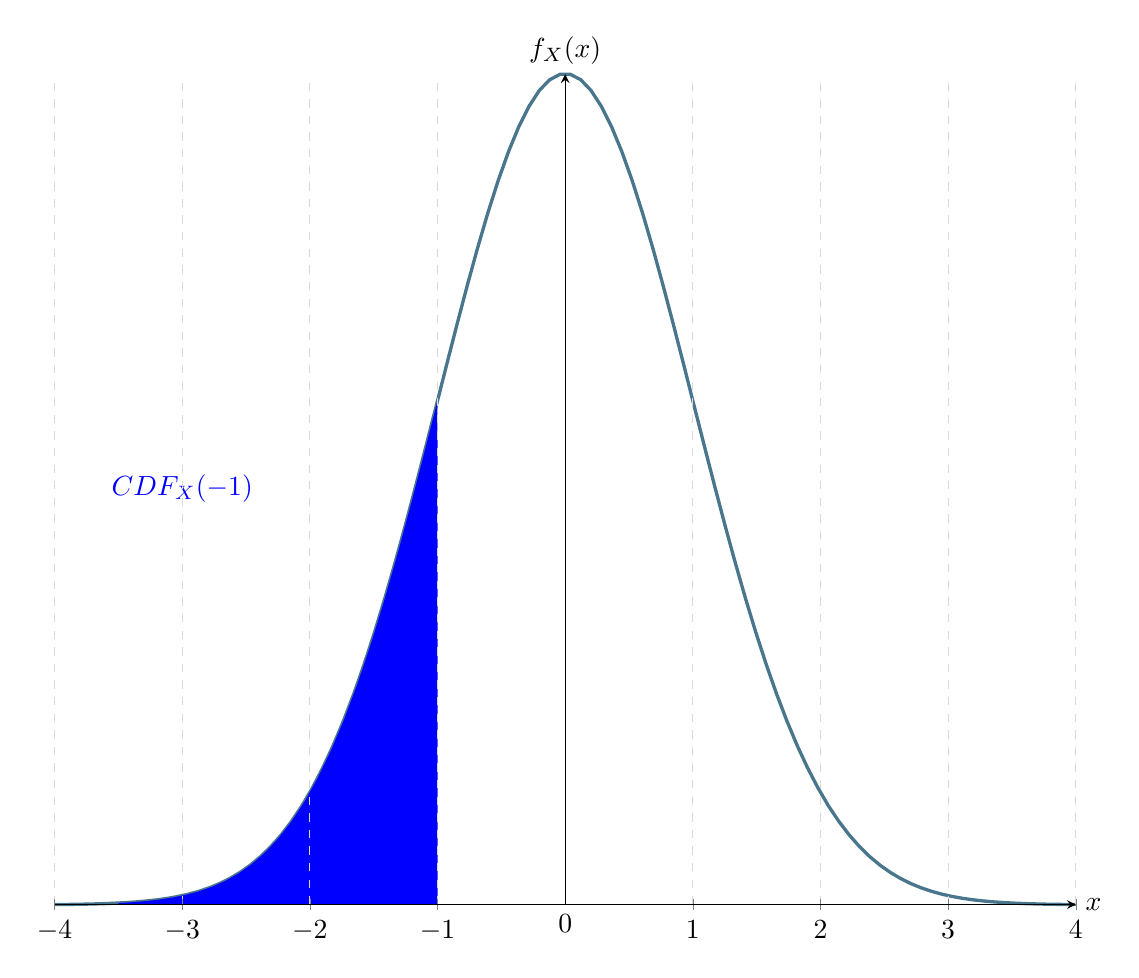
\begin{tikzpicture}
    \begin{axis}[
        domain=-4:4, 
        samples=100, 
        axis lines=middle, 
        xlabel=$x$, 
        ylabel={$f_X(x)$},
        every axis y label/.style={at=(current axis.above origin),anchor=south},
        every axis x label/.style={at=(current axis.right of origin),anchor=west},
        height=1\textwidth, 
        width=1.2\textwidth,
        xtick={-4,-3,...,4},
        ytick=\empty,
        enlargelimits=false, 
        clip=false, 
        axis on top,
        grid = major,
        grid style={dashed, gray!30}
    ]
    % Draw the std normal curve
        \addplot [
            very thick,
            cyan!50!black,
        ] {1/sqrt(2*pi) * exp(-x^2 / 2)};
        \node[below] at (axis cs: 0,0) {$0$};
      % Shade under curve left
  \fill[blue, domain=-3.5:-1, variable=\x] 
    (-3.5, 0) 
    -- plot(\x,{exp(-\x*\x/2)/sqrt(2*pi)}) 
    -- (-1, 0) 
    -- cycle;
  % Labels for areas
  \node at (-3,0.2) {\textcolor{blue}{$CDF_X(-1)$}};
    \end{axis}
\end{tikzpicture}
\end{figure}

\end{columns}

\end{frame}

%% SLIDE #{} %%%%%%%%%%%%%%%%%%%%%%%%%%
\begin{frame}
\frametitle{CDFs for Symmetric Distributions with $\mu_X=0$}

\begin{columns}

\column{0.5\textwidth}

\begin{figure}[ht]
\centering
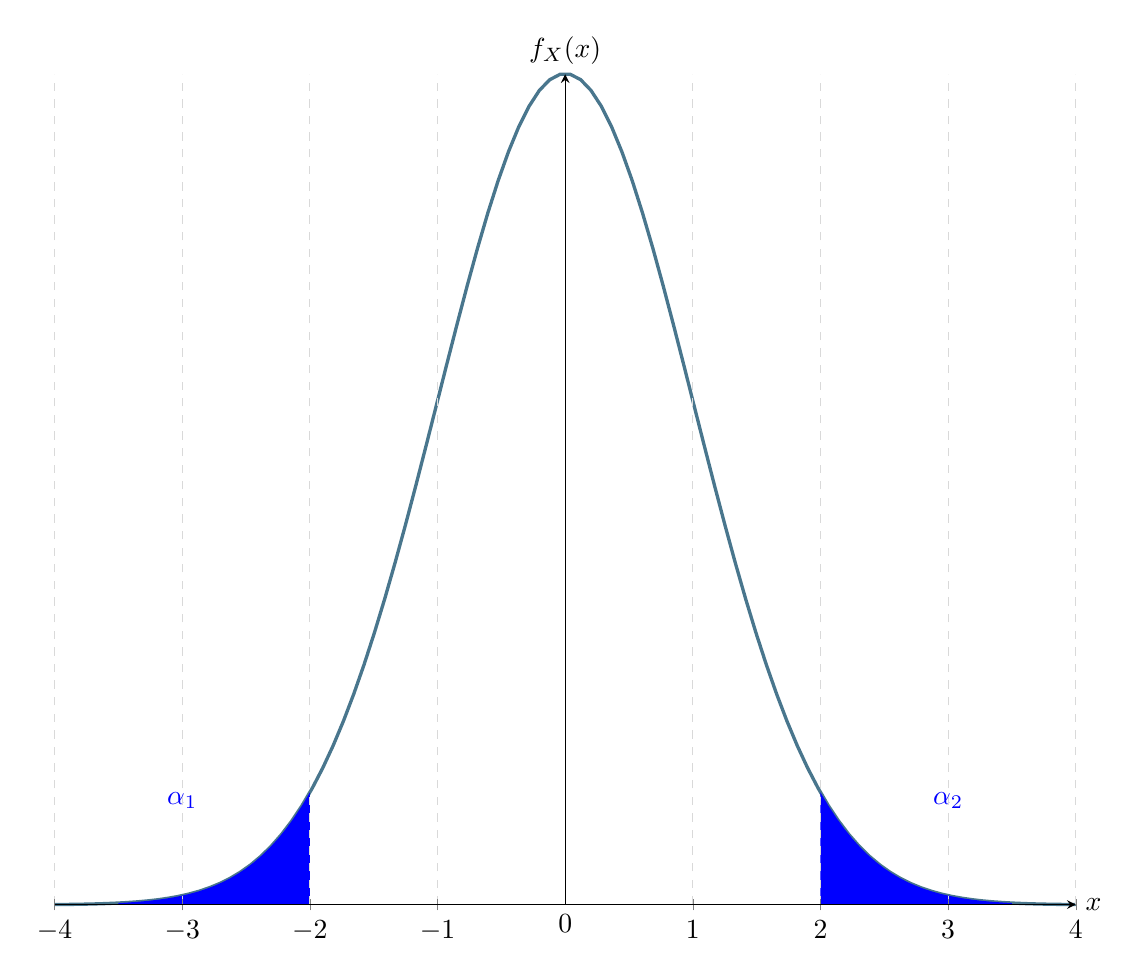
\begin{tikzpicture}
    \begin{axis}[
        domain=-4:4, 
        samples=100, 
        axis lines=middle, 
        xlabel=$x$, 
        ylabel={$f_X(x)$},
        every axis y label/.style={at=(current axis.above origin),anchor=south},
        every axis x label/.style={at=(current axis.right of origin),anchor=west},
        height=1\textwidth, 
        width=1.2\textwidth,
        xtick={-4,-3,...,4},
        ytick=\empty,
        enlargelimits=false, 
        clip=false, 
        axis on top,
        grid = major,
        grid style={dashed, gray!30}
    ]
    % Draw the std normal curve
        \addplot [
            very thick,
            cyan!50!black,
        ] {1/sqrt(2*pi) * exp(-x^2 / 2)};
        \node[below] at (axis cs: 0,0) {$0$};
      % Shade under curve left
  \fill[blue, domain=-3.5:-2, variable=\x] 
    (-3.5, 0) 
    -- plot(\x,{exp(-\x*\x/2)/sqrt(2*pi)}) 
    -- (-2, 0) 
    -- cycle;
  % Shade under curve right
  \fill[blue, domain=2:3.5, variable=\x] 
    (2, 0) 
    -- plot(\x,{exp(-\x*\x/2)/sqrt(2*pi)}) 
    -- (3.5, 0) 
    -- cycle;
  % Labels for areas
  \node at (-3,0.05) {\textcolor{blue}{$\alpha_1$}};
  \node at (3,0.05) {\textcolor{blue}{$\alpha_2$}};
    \end{axis}
\end{tikzpicture}
\end{figure}
  \pause

\vspace{1em}
\column{0.5\textwidth}
\textbf{Symmetry and CDF}
\begin{itemize}
    \setlength{\itemsep}{-12pt} % adj distance between items
  \item Assume $a>0$. For a symmetric PDF (or PMF) with $\mu_X=0$, the following holds:
  \pause
  \[
  P(X \leq -a) = P(X \geq a)
  \]
  \vspace{-1.0em}
  \item Hence:
  \pause
  \[
  CDF_X(-a) = 1 - CDF_X(a)
  \]
  \pause
\end{itemize}
\end{columns}

\begin{itemize}
    \item e.g., if $x$ is a Std. Normal, then: 
    $$0.023 = \alpha_1 = CDF_X(-2) = 1-CDF_X(2) = \alpha_2 = 0.023$$
\end{itemize}
\small 

\end{frame}

%% SLIDE #{} %%%%%%%%%%%%%%%%%%%%%%%%%%
\begin{frame}
\frametitle{Symmetrical Distribution of a Discrete Random Variable}

\begin{columns}

\column{0.4\textwidth}
\footnotesize
\begin{table}[h!]
    \centering
    \begin{tabular}{|c|c|c|}
    \hline
    $\bm{X}$ & $\bm{p_X(x)}$ & $\bm{CDF_X(x)}$  \\
    \hline
    1 & 0.1 & 0.1 \\
    2 & 0.15 & 0.25  \\
    3 & 0.25 & 0.5  \\
    4 & 0.25 & 0.75  \\
    5 & 0.15 & 0.9  \\
    6 & 0.1 & 1.0  \\
    \hline
    \end{tabular}
\end{table}
  \pause

\column{0.6\textwidth}
\begin{figure}[ht]
\centering
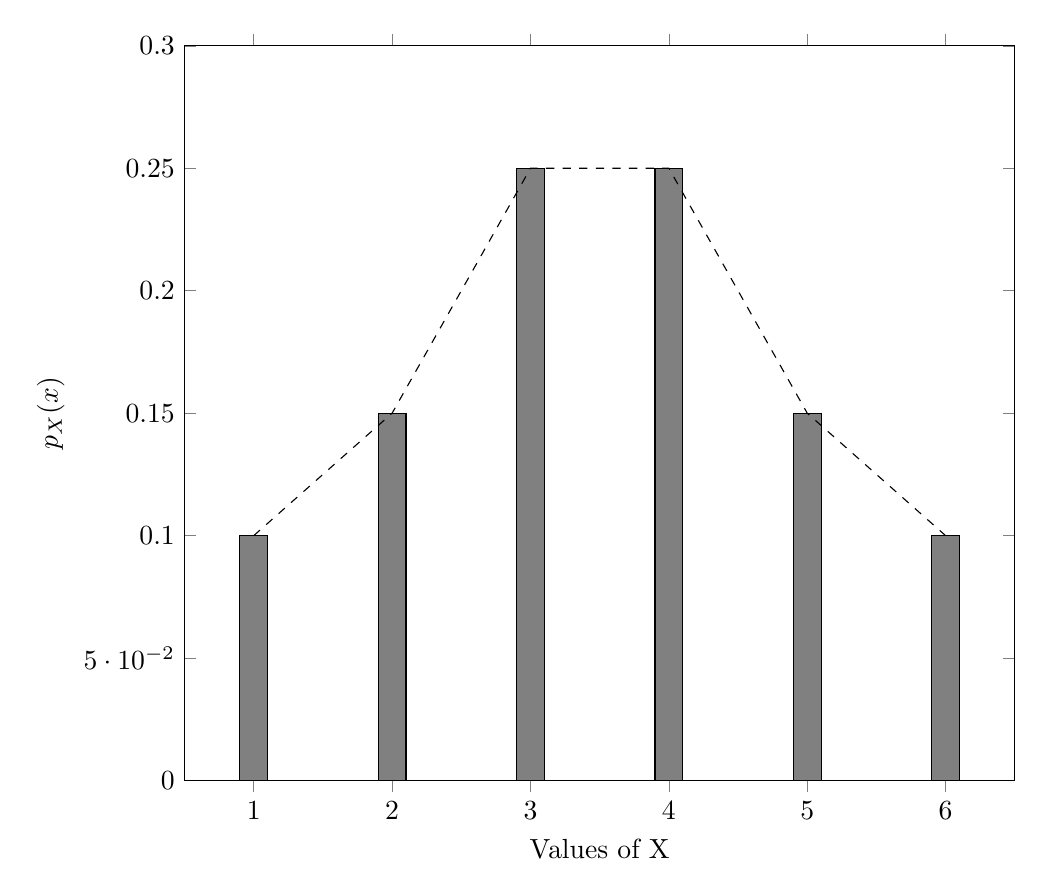
\begin{tikzpicture}
\begin{axis}[
    ybar,
    symbolic x coords={1,2,3,4,5,6},
    xtick=data,
    ymin=0, ymax=0.3,
    ylabel={$p_X(x)$},
    xlabel={Values of X},
    height=0.9\textwidth, 
    width=1\textwidth
]
\addplot[fill=gray] coordinates {(1,0.1) (2,0.15) (3,0.25) (4,0.25) (5,0.15) (6,0.1)};
\draw[dashed] (axis cs:1,0.1) -- (axis cs:2,0.15) -- (axis cs:3,0.25) -- (axis cs:4,0.25) -- (axis cs:5,0.15) -- (axis cs:6,0.1);
\end{axis}
\end{tikzpicture}
\end{figure}

\end{columns}

\end{frame}

\end{document}


\begin{frame}{CDF of the Standard Normal}
    - Teach how to compute probabilities with the standard normal    
\end{frame}


~~~~ IDEAS: ~~~~~~~~~~~~~~~~~~~~~~~~~~~~~~~~~~~~~~~~~~

Changes:
- Remove the useless slides on CDF(-1)
- Update slides: Do a more weird PMF with 7 values. Actually, let's do a poisson. Do not show the PMF values, just CDF.
- Add a slide using the probability rules using CDFs to compute probabilities given the CDF table. 

add to brightspace:
https://www.tiktok.com/@veritasium/video/7352561248824806698

- emergence of the normal distribution
https://www.youtube.com/watch?v=xuehJYGoflE

https://onlinestatbook.com/2/normal_distribution/history_normal.html

https://medium.com/@will.a.sundstrom/the-origins-of-the-normal-distribution-f64e1575de29

https://www.tandfonline.com/doi/abs/10.1080/0025570X.2006.11953386

